% 02.06.2016 12:00 CET last changed by a.holzinger
% General Template for LNCS and LNAI contributions based on llncs, adapted by ah
% Many thanks to the TRS team
% In case of using eps compile via 1) TeXify and then proceed with 2) dvi2pdf
%
\documentclass{llncs}
\usepackage{float}

\usepackage[dvips]{graphicx}
\usepackage[ruled,vlined]{algorithm2e}
\usepackage{amsfonts}
\usepackage{amssymb}
\usepackage{amsmath}
\usepackage{mathtools}

\providecommand{\abs}[1]{\lvert#1\rvert}
\providecommand{\norm}[1]{\lVert#1\rVert}

\usepackage{calc}
\usepackage{subfigure}

\usepackage{color}
\usepackage{soul}
\usepackage{comment}

\newtheorem{prop}{Property}

\newenvironment{Bitemize}{\renewcommand\labelitemi{\textbullet}\begin{itemize}}{\end{itemize}}

\begin{document}

\title{The right to be forgotten:\\
Towards Machine Learning on perturbed knowledge bases}

\author{Bernd Malle\inst{1}\inst{2}, Peter Kieseberg\inst{1}\inst{2}, Edgar Weippl\inst{2}, Andreas Holzinger\inst{1}}

\institute{Holzinger Group HCI-KDD \\
Institute for Medical Informatics, Statistics \& Documentation\\
            Medical University Graz, Austria\\
            \texttt{b.malle@hci-kdd.org}
\and
SBA Research gGmbH, Favoritenstraße 16, 1040 Wien \\
			\texttt{PKieseberg@sba-research.org}
}
	
\maketitle

% ==================================
%				ABSTRACT
% ==================================
\begin{abstract}


Today's increasingly complex information infrastructures represent the basis of any data-driven industries which are rapidly becoming the 21st century's economic backbone. The sensitivity of those infrastructures to disturbances in their knowledge bases is therefore of crucial interest for companies, organizations, customers and regulating bodies. This holds true with respect to the direct provisioning of such information in crucial applications like clinical settings or the energy industry, but also when considering additional insights, predictions and personalized services that are enabled by the automatic processing of those data. In the light of new EU Data Protection regulations applying from 2018 onwards which give customers the right to have their data deleted on request, information processing bodies will have to react to these changing jurisdictional (and therefore economic) conditions. Their choices include a re-design of their data infrastructure as well as preventive actions like anonymization of databases per default. Therefore, insights into the effects of perturbed / anonymized knowledge bases on the quality of machine learning results are a crucial basis for successfully facing those future challenges. In this paper we introduce a series of experiments we conducted on applying four different classifiers to an established dataset, as well as several distorted versions of it and present our initial results.


\medskip

\textbf{Keywords}: Machine learning, knowledge bases, right to be forgotten, perturbation, anonymization, k-anonymity, SaNGreeA, information loss, structural loss, cost weighing vector, interactive machine learning


\end{abstract}

\renewcommand{\thesubfigure}{\thefigure.\arabic{subfigure}}
\makeatletter
\renewcommand{\p@subfigure}{}
\renewcommand{\@thesubfigure}{\thesubfigure:\hskip\subfiglabelskip}
\makeatother


% ==================================
%			INTRODCUTION
% ==================================
\section{Introduction and Motivation for Research}

Privacy aware machine learning \cite{DuchiJordan:2014:PrivacyAwareLearning} is an issue of increasing importance, fostered by anonymization concepts like k-anonymity \cite{Samarati:2001:kAnonymity}, in which a record is released only if it is indistinguishable from $k$ other entities in the data set. However, k-anonymity is highly dependent on spatial locality in order to effectively implement the technique in a statistically robust way, and in arbitrarily high dimensions data becomes sparse, hence, the concept of spatial locality is not easy to define. Consequently, it becomes difficult to anonymize the data without an unacceptably high amount of information loss \cite{Aggarwal:2005:kAnonymity}. Therefore, the problem of k-anonymization is on the one hand NP-hard, on the other hand the quality of the result obtained can be measured at the given factors: \emph{k-anonymity} means that attributes are suppressed or generalized until each row in a database is identical with at least $k-1$ other rows \cite{Sweeney:2002:k-Anonymity}; \emph{l-diversity} as extension of the k-anonymity model reduces the granularity of the data representation by generalization and suppression so that any given record maps onto at least $k$ other records in the data \cite{MachanavajjhalaEtAl:2007:l-Diversity}; \emph{t-closeness} is a refinement of l-diversity by reducing the granularity of a data representation, and treating the values of an attribute distinctly by taking into account the distribution of data values for that attribute \cite{LiEtAl:2007:t-closeness}; and \emph{delta-presence}, which links the quality of anonymization to the risk posed by inadequate anonymization \cite{NergizClifton:2010:Delta-Presence}, but not with regard to the actual security of the data, i.e., the re-identification through an attacker. For this purpose, certain assumptions about the background knowledge of the hypothetical enemy must be made. In this work, we are going to measure the effects of the anonymization of knowledge bases on the performance of machine learning algorithms in order to give valuable feedback to data holders and anonymization providers.

Another challenge for data processing entities is increasingly imposed on them by the law. At least within the European Union, where a new Data Protection Reform will apply from 2018 onwards, customers are given a \textit{right to be forgotten}, which means that an organization is obligated to remove a customer's personal data upon request. Since information in a modern, data driven infrastructure is not only usable for the customer herself, but also constitutes the basis for machine learning algorithms providing better insights and services, this information loss might be problematic, if only in competition with companies / organizations which do not fall under such jurisdiction. The ability to quantify the effects of information loss by erasure of sensitive data is therefore of great importance and the other core focus of our work.


% ==================================
%			BASIC CONCEPTS
% ==================================
\section{Scenarios of incurring information loss in datasets}


\subsection{Selective perturbation}

Within a modern information infrastructure, several layers of data storage and processing might be affected by the \textit{right to be forgotten}. The first and probably most benign impact would be the one on so-called \textit{Front-End} databases; those are customer-facing databases on the backend which handle the bulk of day-to-day data transmissions and contain the customer's data in full detail. Erasing a data entry from this Front-end is therefore simple and of manageable consequences. 

The second layer impacted by data erasure are archival and backup systems, which are necessary in case of failures on the Front-end. Although data erasure does not pose any technical problem here either, it is necessary to consider it on an organizational level in order to not inadvertently re-introducing already "forgotten" items.

Significant problems are to be expected when executing selective data erasure on statistical databases or knowledge bases prepared for machine-learning. Both kinds of DBs will usually not hold the original user information but merely statistically relevant fragments of it; this difficulty is compounded by the fact that in many cases it might not be technically necessary to even store a link to the original data. In such cases is it not only impossible to delete the relevant fragments from such data stores (not to mention the statistical / parametric results obtained by algorithms working on them), but the whole databases might have to be recreated upon every user deletion request. It is therefore absolutely crucial to have an insight into the results of potential data perturbation, if only to be able to redesign (parts of) an information infrastructure.


\subsection{Tabular anonymization}
\label{ssect:tab_anonym}

Figure~\ref{fig:anon_categories} illustrates the original tabular concept of anonymization: Given an input table with several columns, we will in all probability encounter three different categories of data:

\begin{itemize}
	\item \textbf{Personal identifiers} are data items which directly identify a person without having to cross-reference or further analyze them. Examples are first and last names, but even more so an (email) address or social security number (SSN). As personal identifiers are dangerous and cannot be generalized (see Figure~\ref{fig:gen_hierarchy}) in a meaningful way (e.g. one could generalize an email address by only retaining the mail provider fragment, but the result would not yield much usable information), this category of data is usually removed. The table shows this column in a red background color.
	\item \textbf{Sensitive data,} also called 'payload', which is the kind of data we want to convey for statistics or research purposes. Examples for this category would be disease classification, drug intake or personal income level. This data shall be preserved in the anonymized dataset and can therefore not be deleted or generalized. The table shows this column in a green background color.
	\item \textbf{Quasi identifiers (QI's)}, colored in the table with an orange background, are data that in themselves do not directly reveal the identity of a person, but might be used in aggregate to reconstruct it. For instance, \cite{sweeney2002k} mentioned that 87\% of U.S. citizens in 2002 had reported characteristics that made them vulnerable to identification based on just the 3 attributes \textit{zip code}, \textit{gender} and \textit{date of birth}. But although this data can be harmful in that respect, it might also hold vital information for the purpose of research (e.g. zip code could be of high value in a study on disease spread). The the actual point of all anonymization efforts is therefore to generalize this kind of information, which means to lower its level of granularity. As an example, one could generalize the ZIP codes 41074, 41075 and 41099 to an umbrella version 410**, as shown in Figure~\ref{fig:anonymized_clusters}.
\end{itemize}

\begin{figure}[!t]
	\begin{center}
		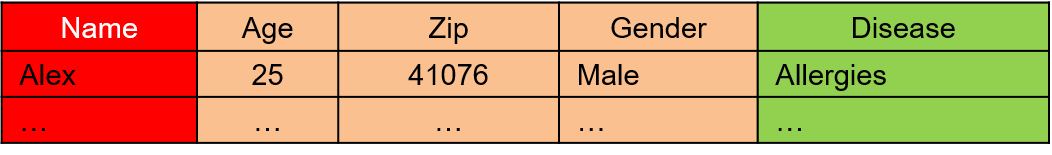
\includegraphics[width=\textwidth]{figures/anonym/3typesofdata}
		\caption{The three types of data considered in (k-)anonymization}
		\label{fig:anon_categories}
	\end{center}
\end{figure}

As described in \cite{ciriani2007kappa}, k-anonymization requires that in each data release every combination of values of quasi-identifiers must be identical to at least $k-1$ other entries in that release, which can be seen as a clustering problem with each cluster's (also called \textit{equivalence class}) quasi-identifier state being identical for every data point. This can be achieved via suppression and generalization, where suppression means simply deletion, whereas in generalization we try to retain some usable value.

The process of generalization works through a concept called \textit{generalization hierarchies}, which form a tree, whose root denotes the most general value available for an attribute (usually the 'all' value) and then branches to more and more specific occurrences, with its leafs representing the set of exact, original values (see Figure~\ref{fig:gen_hierarchy}). In generalizing the original input value, one traverses the tree from the leaf level upwards until a prerequisite is fulfilled. Usually, this comes in the form of the k-anonymity requirement, so that we want to find a group of other data entries whose generalized QI's match the data point being processed.

\begin{figure}[!t]
	\begin{center}
		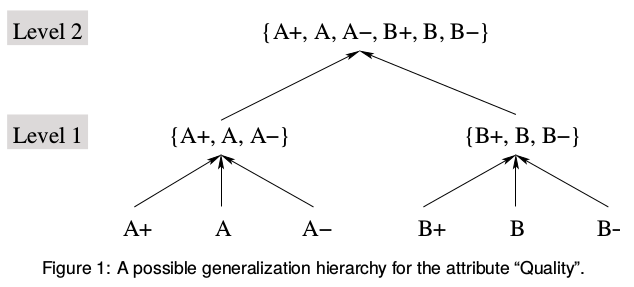
\includegraphics[width=\textwidth]{figures/anonym/gen_hierarchy}
		\caption{Example of a typical generalization hierarchy}
		\label{fig:gen_hierarchy}
		\small
		taken from \cite{aggarwal2005approximation}
	\end{center}
\end{figure}


Each level of generalization involves a certain cost in information loss, so we do not want to construct our clusters in any random sequence but minimize the overall information loss \cite{aggarwal2005approximation}. This makes k-anonymization an NP-hard problem due to an exponential number of possible generalized QI combinations.

\begin{figure}[!t]
	\centering
	\begin{minipage}[b]{0.535\textwidth}
		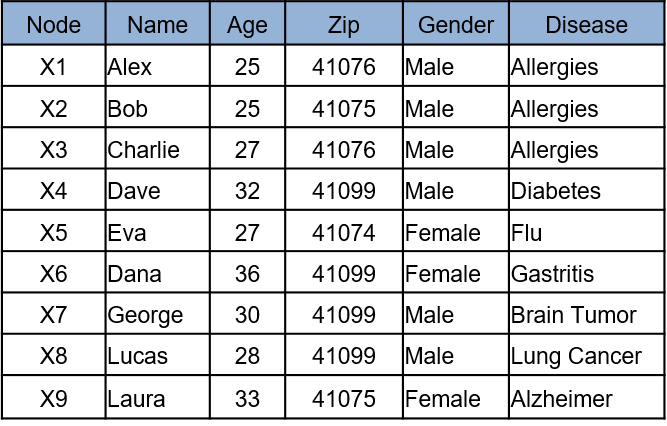
\includegraphics[width=\textwidth]{figures/anonym/k_anon_input}
	\end{minipage}
	\hfill
	\begin{minipage}[b]{0.448\textwidth}
		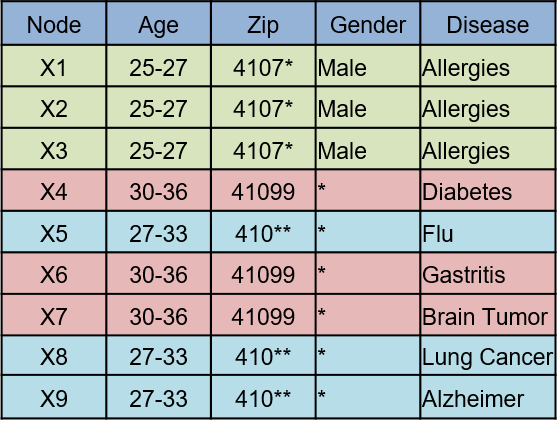
\includegraphics[width=\textwidth]{figures/anonym/k_anon_output}
	\end{minipage}
	\caption{Tabular anonymization: input table and anonymization result}
	\label{fig:anonymized_clusters}
\end{figure}


\subsection{Graph (social network) anonymization}
\label{ssect:graph_sn_anon}

Hitherto we were solely concerned with tabular data; however, as social networks have gained huge popularity over the previous decade, and are widely applicable in other areas as well, the question of how to efficiently anonymize networks has gained ever more significance over the years.

As a start, one could see a graph just as a collection of nodes, where each node contains some kind of feature vector, akin to the row in a data table. Adopting that view, we could be tempted to simply ignore the existence of edges and apply some kind of algorithm suitable to the anonymization of tabular data. The main problem with this however lies in the fact that the structural environment of a node (the constellation of its neighbors within the greater network) provides some additional information. That is, even if we successfully (k-)anonymize the feature vectors of a graph according to the methods described in the previous chapter, we still run the risk of too much information remaining in the form of a known local subgraph structure.

Consider Figure~\ref{fig:anon_sn_problem} for example, in which the nodes of a graph have already been k-anonymized into groups of size 3 and 7, respectively. In this figure, local subgraphs b) and c) are actually (3)-anonymized, because as each node has the exact same local neighborhood structure, the additional information of a node possessing a degree of 0 (or 2) is of no additional value. For local subgraphs a) and d) on the other hand, the additional information of a node being of degree (x) has the potential to reveal its identity, meaning it is not indistinguishable from its neighbors within the equivalence class any more.

\begin{figure}[!t]
	\begin{center}
		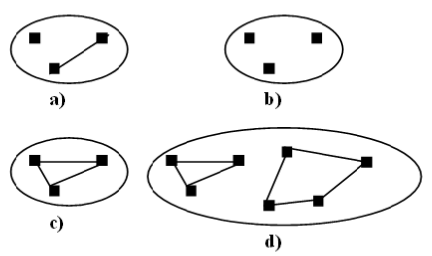
\includegraphics[width=0.8\textwidth]{figures/anonym/sn_problem}
		\caption{Local subgraph neighborhoods as additional anonymization obstacle.}
		\label{fig:anon_sn_problem}
	\end{center}
	\small
	(Example taken from \cite{campan2009data}.)
\end{figure}


Several methods have been proposed to make re-identification of nodes in anonymized social graphs harder.	\cite{chester2011k} for example introduce the idea of vertex addition to labeled and unlabeled datasets. While an algorithm on the former remains NP complete, they provide an efficient ($O(nk)$) algorithm for unlabeled data. Experimenting on several well known datasets, they show that commonly-studied structural properties of the network, such as clustering coefficient, are only minorly distorted by their anonymization procedure.

Person re-identification is both a hard and important problem in many different domains and is challenging. Most approaches aim to model and extract distinctive and reliable features. However, seeking an optimal and robust similarity measure that quantifies a wide range of features against realistic conditions from a distance is still an open and unsolved problem for person re-identification techniques \cite{Zheng:2013:reidentification}. 

In order to develop protection techniques in social networks it is necessary to consider three aspects \cite{Zhou:2008:SurveyAnonNetwork}: 1) the privacy information which may be
under attack; 2) the background knowledge that an adversary may use to attack the privacy
of target individuals; and 3) a specification of the usage of the published social network data so that an anonymization method can try to retain the utility of the data as much as possible whilst the privacy is preserved. 

The authors of \cite{kapron2011social} take the approach of adding edges to an edge-labeled graph like the Netflix movie database (with users and movies being nodes and edge weights representing movie ratings). They define tables as bipartite graphs and prove NP-hardness for the problems of neighborhood anonymity, i-hop anonymity and k-symmetry anonymity.

Campan \cite{campan2009data}, whose local subgraph problem we already encountered, proposed a solution in the form of a greedy clustering algorithm which takes into account not only the information loss incurred by generalizing features of nodes, but also introducing a structural loss function based on the local neighborhood within an equivalence class (and between them). The author of this thesis implemented that approach utilizing GraphiniusJS and will demonstrate the algorithm in Section~\ref{ssect:algorithm} as well as the anonymized results in Section~\ref{sect:results}.


% ==================================
%				EXPERIMENTS
% ==================================
\section{Experiments}
\label{sect:experiments}

The following sections will describe our series of experiments in detail, encompassing the data source selected, the algorithm used as well as a description of the overall process employed to obtain our results.


\subsection{Data} 
\label{ssect:data}

As input data we chose the adults dataset from the UCI Machine Learning repository which was generated from US census data of 1994 and contains approximately 32,000 entries; from those 30,162 were selected after preprocessing. Of the attributes (data columns) provided only one was deleted because it was also represented by a column containing its numerical mapping (education $=>$ education\_num). Figure~\ref{fig:adult_original_distribution} shows the attribute value distribution of the original input dataset with the exception of the sample weights.


\begin{figure}[!t]
	\begin{center}
    \hspace*{-0.8cm}
		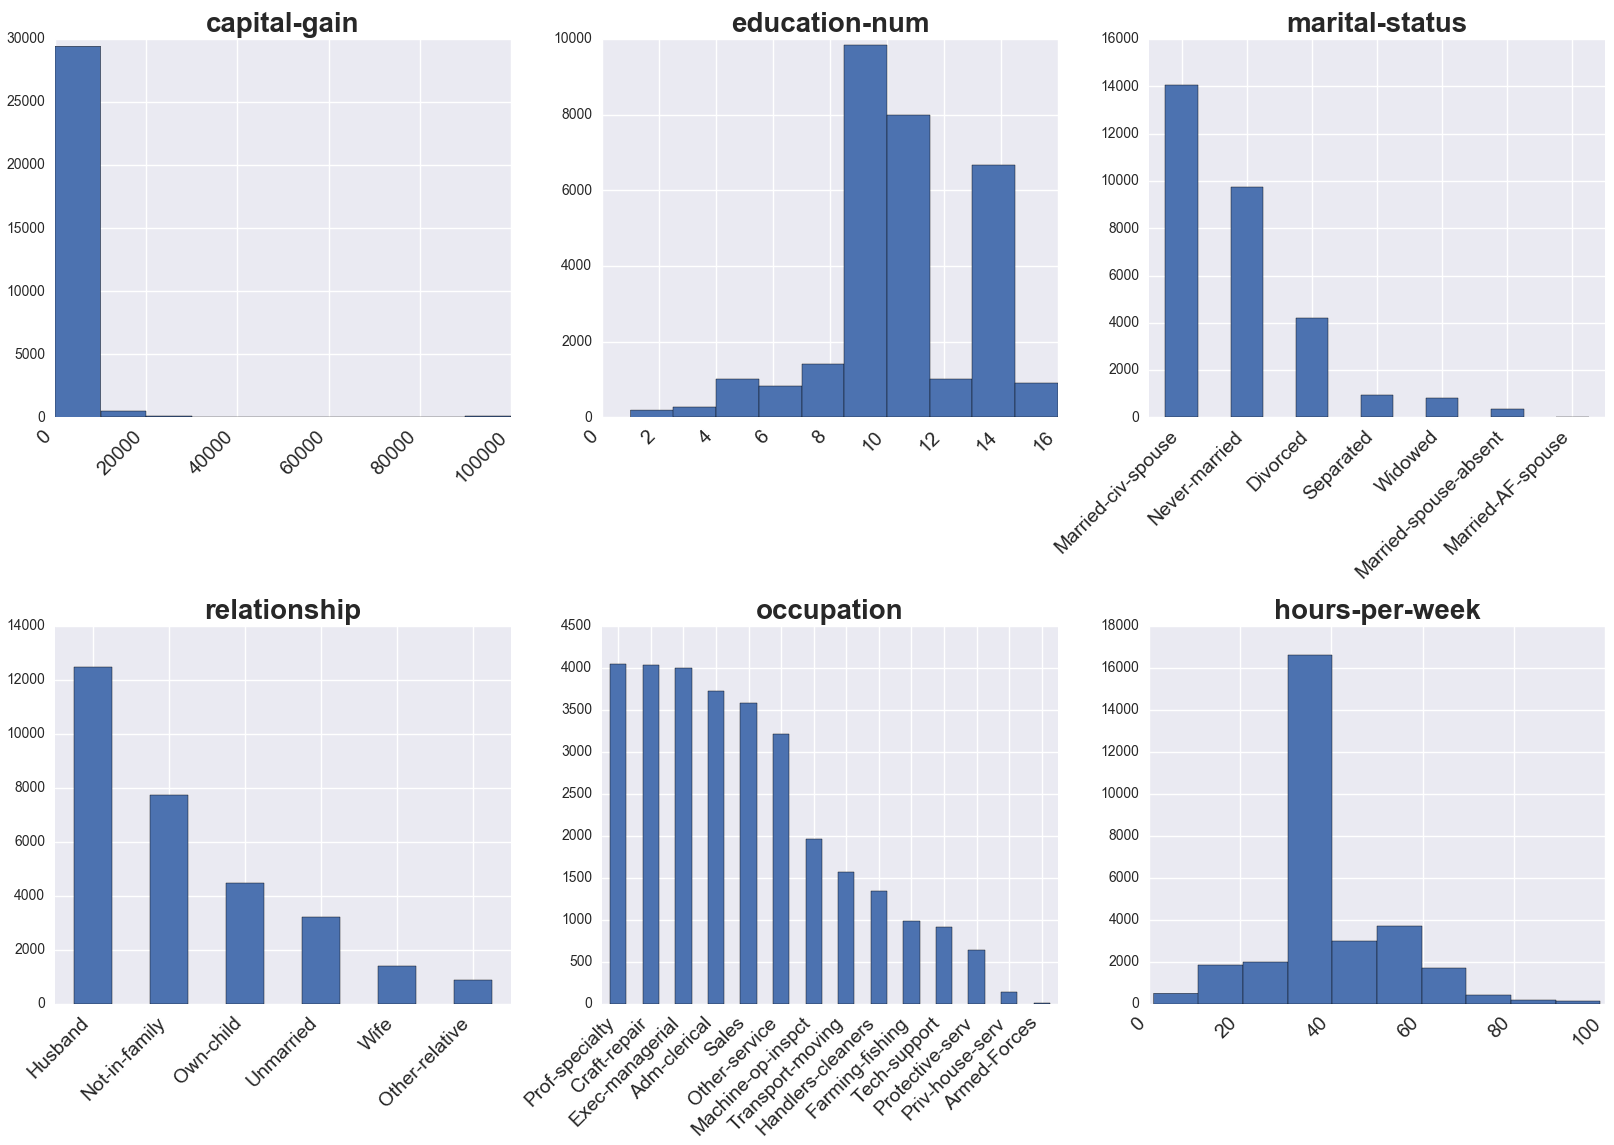
\includegraphics[width=1.1\textwidth]{figures/experiment/dist_initial_small}
		\caption{Initial distribution of the most important (w.r.t. classifier result quality) data columns of the adult dataset}
		\label{fig:adult_original_distribution}
	\end{center}
\end{figure}

As one can see, there are several attributes with one value clearly dominating the others; \textit{native-country} being the most prominent example with the entry for the United States dwarfing all other countries (which comes as no surprise given the data origin). As anonymization generalizes different countries together if necessary, it was interesting for the author to see how these distributions would change under a relatively large k-factor. Figure~\ref{fig:adult_anonymized_distribution} shows the same attribute distribution with its values anonymized by a factor of $k=19$. Although the dominance of the United states was successfully "broken" by this method, in several instances the \textit{generalized-to-all}-value (*) now skews the data set even more. Apart from the expected generalization information loss this is another reason why one would assume worse results from a machine learning classifier applied to an anonymized dataset.

\begin{figure}[!t]
	\begin{center}
    	\hspace*{-0.8cm}
		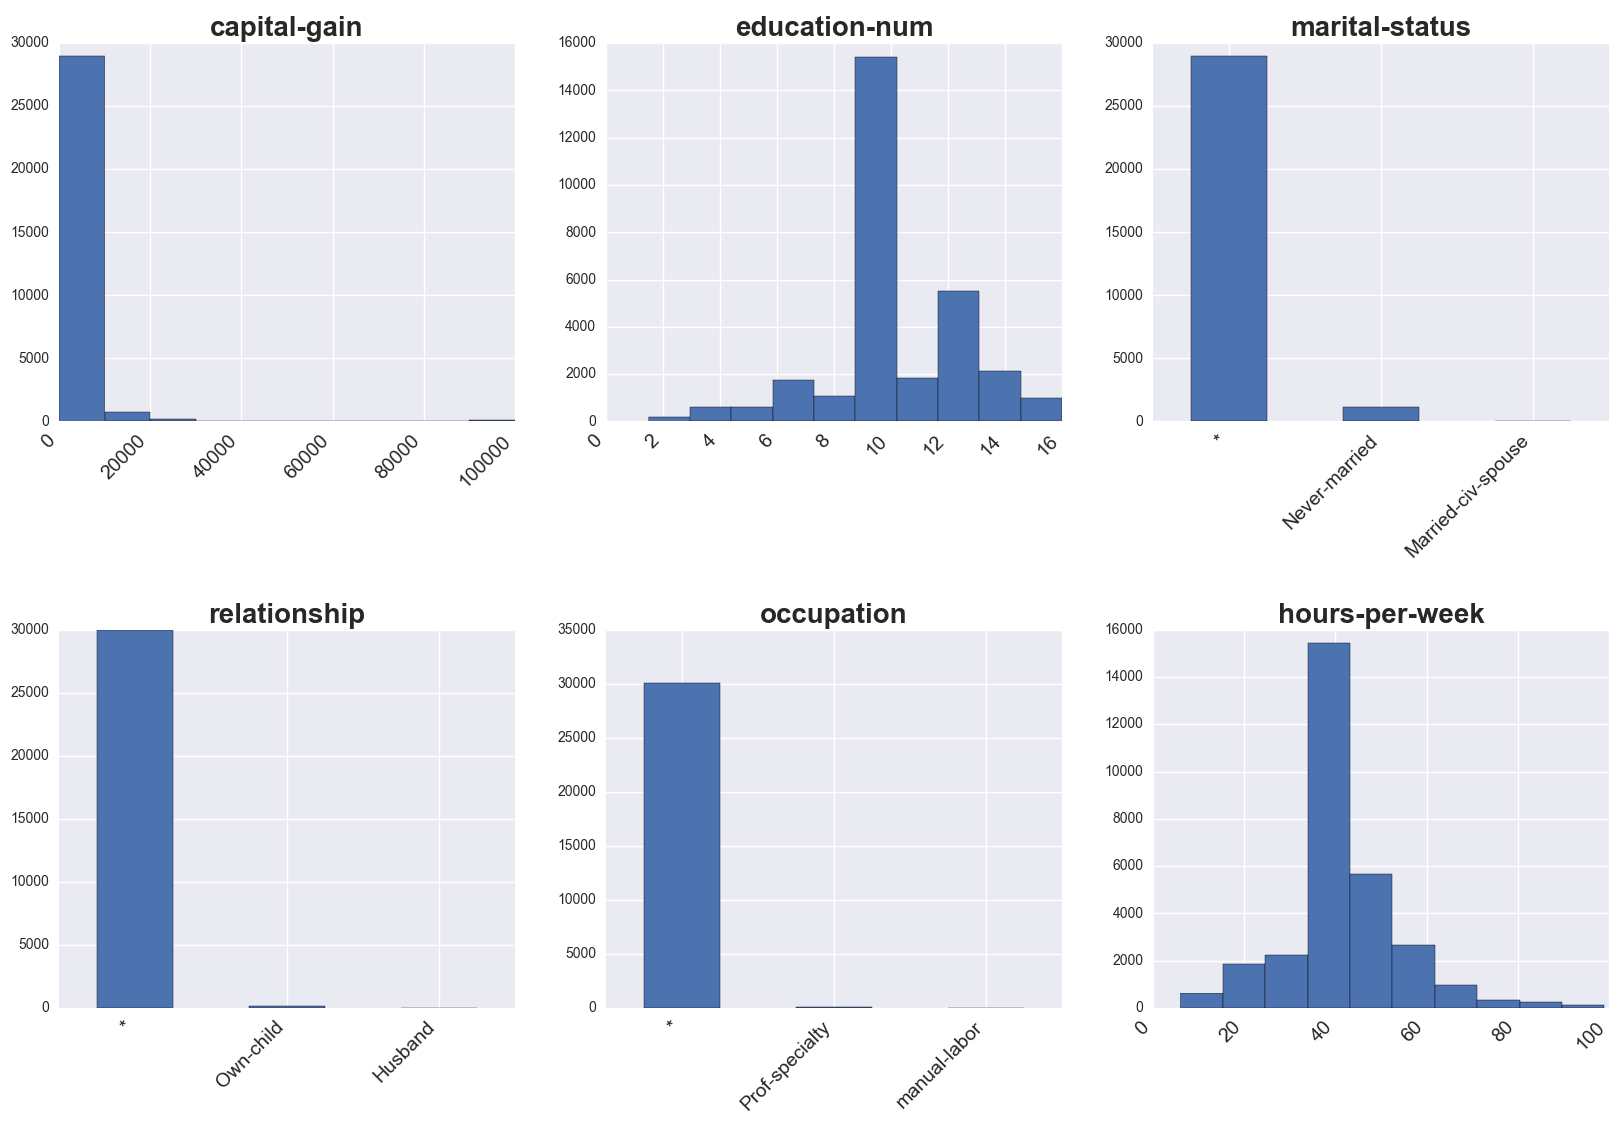
\includegraphics[width=1.1\textwidth]{figures/experiment/dist_anonym_small}
		\caption{Anonymized distribution of the most important (w.r.t. classifier result quality) data columns of the adult dataset, anonymization factor of k=19, equal weight for each attribute.}
		\label{fig:adult_anonymized_distribution}
	\end{center}
\end{figure}



\subsection{Algorithm}
\label{ssect:algorithm}

SaNGreeA stands for \textit{Social network greedy clustering} and was introduced by \cite{campan2009data}. In addition to 'clustering' nodes of a graph according to the minimum general information loss (GIL) incurred as described in Section~\ref{ssect:tab_anonym}, this algorithm also considers the structural information loss (SIL) incurred in assigning a node to a certain cluster. The SIL quantifies the probability of error when trying to reconstruct the structure of the initial graph from its anonymized version.

\begin{equation*}
\begin{split}
\text{GIL}(cl) = \abs{cl} \cdot (\sum_{j=1}^{s} \frac{size(gen(cl)[N_j])}{size(min_{x \epsilon N} (X[N_j]), max_{x \epsilon N} (X[N_j]))} \\ 
+ \sum_{j=1}^{t} \frac{height(\Lambda(gen(cl)[C_j]))}{height(H_{C_j})})    
\end{split}    
\end{equation*}


where:\\
- $\abs{cl}$ denotes the cluster cl's cardinality; \\
- $size([i1,i2])$ is the size of the interval $[i1,i2]$, i.e., $(i2-i1)$; \\
- $\Lambda(w), w \epsilon H_{C_j}$ is the sub-hierarchy of $H_{C_j}$ rooted in $w$; \\
- $height(H_{C_j})$ denotes the height of the tree hierarchy $H_{C_j}$; \\


The total generalization information loss is then given by:
\begin{equation*}
\text{GIL}(G,S) = \sum_{j=1}^{v} \text{GIL}(cl_j)
\end{equation*}
And the normalized generalization information loss by:
\begin{equation*}
\text{NGIL}(G,S) = \frac{\text{GIL}(G,S)}{n \cdot (s+t)}
\end{equation*}

The SIL is composed of two different components: 1) the intra-cluster structural loss, signifying the error probability in trying to reconstruct the original edge distribution within an equivalence class (= anonymized cluster), and 2) the inter-cluster structural loss which represents the error probability in trying to reconstruct the original configuration of edges between two equivalence classes.

For the exact mathematical definitions of SIL \& NSIL the reader is kindly referred to the original paper. Because the structural information loss cannot be computed exactly before the final construction of clusters, the exact computations were replaced by the following distance measures: \\

Distance between two nodes:
\begin{equation*}
\text{dist}(X^i, X^j) = \frac{\abs{\{l|l=1..n \wedge l \ne i,j;b_l^i \ne b_l^j}}{n-2}
\end{equation*}

Distance between a node and a cluster:
\begin{equation*}
\text{dist}(X, cl) = \frac{\sum_{X^j \epsilon cl} \text{dist}(X, X^j) }{\abs{cl}}
\end{equation*}


The algorithm starts with initializing a first cluster by a randomly choosing a node. Then, for every new node encountered, the weighted sum of the above two information loss metrics will yield a certain overall information loss in case the node was added to that cluster - the candidate with minimal information loss is then added to the cluster. This process is repeated until the cluster reaches a certain constraint (e.g. size $ \coloneqq  k $ -factor) upon which another random node is chosen to constitute the next cluster. This procedure is repeated until all nodes have been assigned; if a cluster of size $< k$ should remain, its member nodes are dispersed accordingly.

Since the algorithm does not take all possible node combinations into account, but simply chooses an arbitrary node and compares all the candidates in a loop, the algorithm runs in quadratic time w.r.t. the input size in number of nodes. This worked well within milliseconds for a problem size of a few hundred nodes, but took up to 60 mins. on the whole adult dataset.

In implementing and demonstrating this algorithm, the authors intended to recreate the original paper's experiment. However, as no suitable real-world graph structure was available to the authors at the time of this writing and any artificially generated network would result in dubious results for the classification tasks applied, we decided to leave out the structural component of the algorithm and focus only on the generalization information loss for this paper, leaving the entire approach to future research initiatives.



\subsection{Process}
\label{ssect:process}

To examine the impact of perturbation and anonymization of datasets on the quality of a classification result, we designed the following processing pipeline:

% , \textit{one vs. rest with bagging}

\begin{enumerate}
	\item Taking the original (preprocessed) dataset as input, we transformed its attributes to boolean values, so instead of \textit{native-country $->$ United-States} we considered \textit{United-States $->$ yes / no}.
	% \item A correlation matrix of the resulting binary feature set was computed to get a better feeling for the data (see Figure~\ref{fig:adult_correlation_big}).
	\item We then ran 5 different classifiers on it and computed precision, recall as well as F1 score. The five classifiers used were \textit{gradient boosting}, \textit{random forest}, \textit{logistic regression} and \textit{linear SVC}.
	\item From the obtained results we extracted the 3 attribute values most contributing to a "positive" ($>$50k) result as well as the top 3 attribute values indicating a "negative" ($<=$50k) prediction as depicted in Figure~\ref{fig:adult_important_columns}
	\item For each of these 6 attribute values, we subsequently deleted a specific percentage of data rows containing that value from the original dataset, resulting in 30 reduced datasets. The 5 percentages used were $0.2$, $0.4$, $0.6$, $0.8$ as well as $1.0$.
	\item To each of those datasets we re-applied the five chosen classifiers successively and recorded the respective impact on the quality of the classification result. The results can be seen in Figure~\ref{fig:adult_results_perturbation_top} and Figure~\ref{fig:adult_results_perturbation_bottom}.
	\item In order to measure the effects of k-anonymization on classifier performance, we used the SaNGreeA's GIL component described in the following section to generate datasets with a k-factor of $k=3$, $k=7$, $k=11$, $k=15$ as well as $k=19$. Furthermore, we used each of these settings with 3 different weight vectors: 1) equal weights for all attributes, 2) age information preferred ($\omega(age)=0.88$, $\omega(other\_attributes)=0.01$) and 3) race information preferred ($\omega(race)=0.88$, $\omega(other\_attributes)=0.01$). We then re-executed all classifiers on the resulting 15 datasets and recorded the respective results, which can be seen in Figure~\ref{fig:adult_results_anonymization}.
\end{enumerate}


% \begin{figure}[!t]
%	\begin{center}
%    	\hspace*{-1.5cm}
%		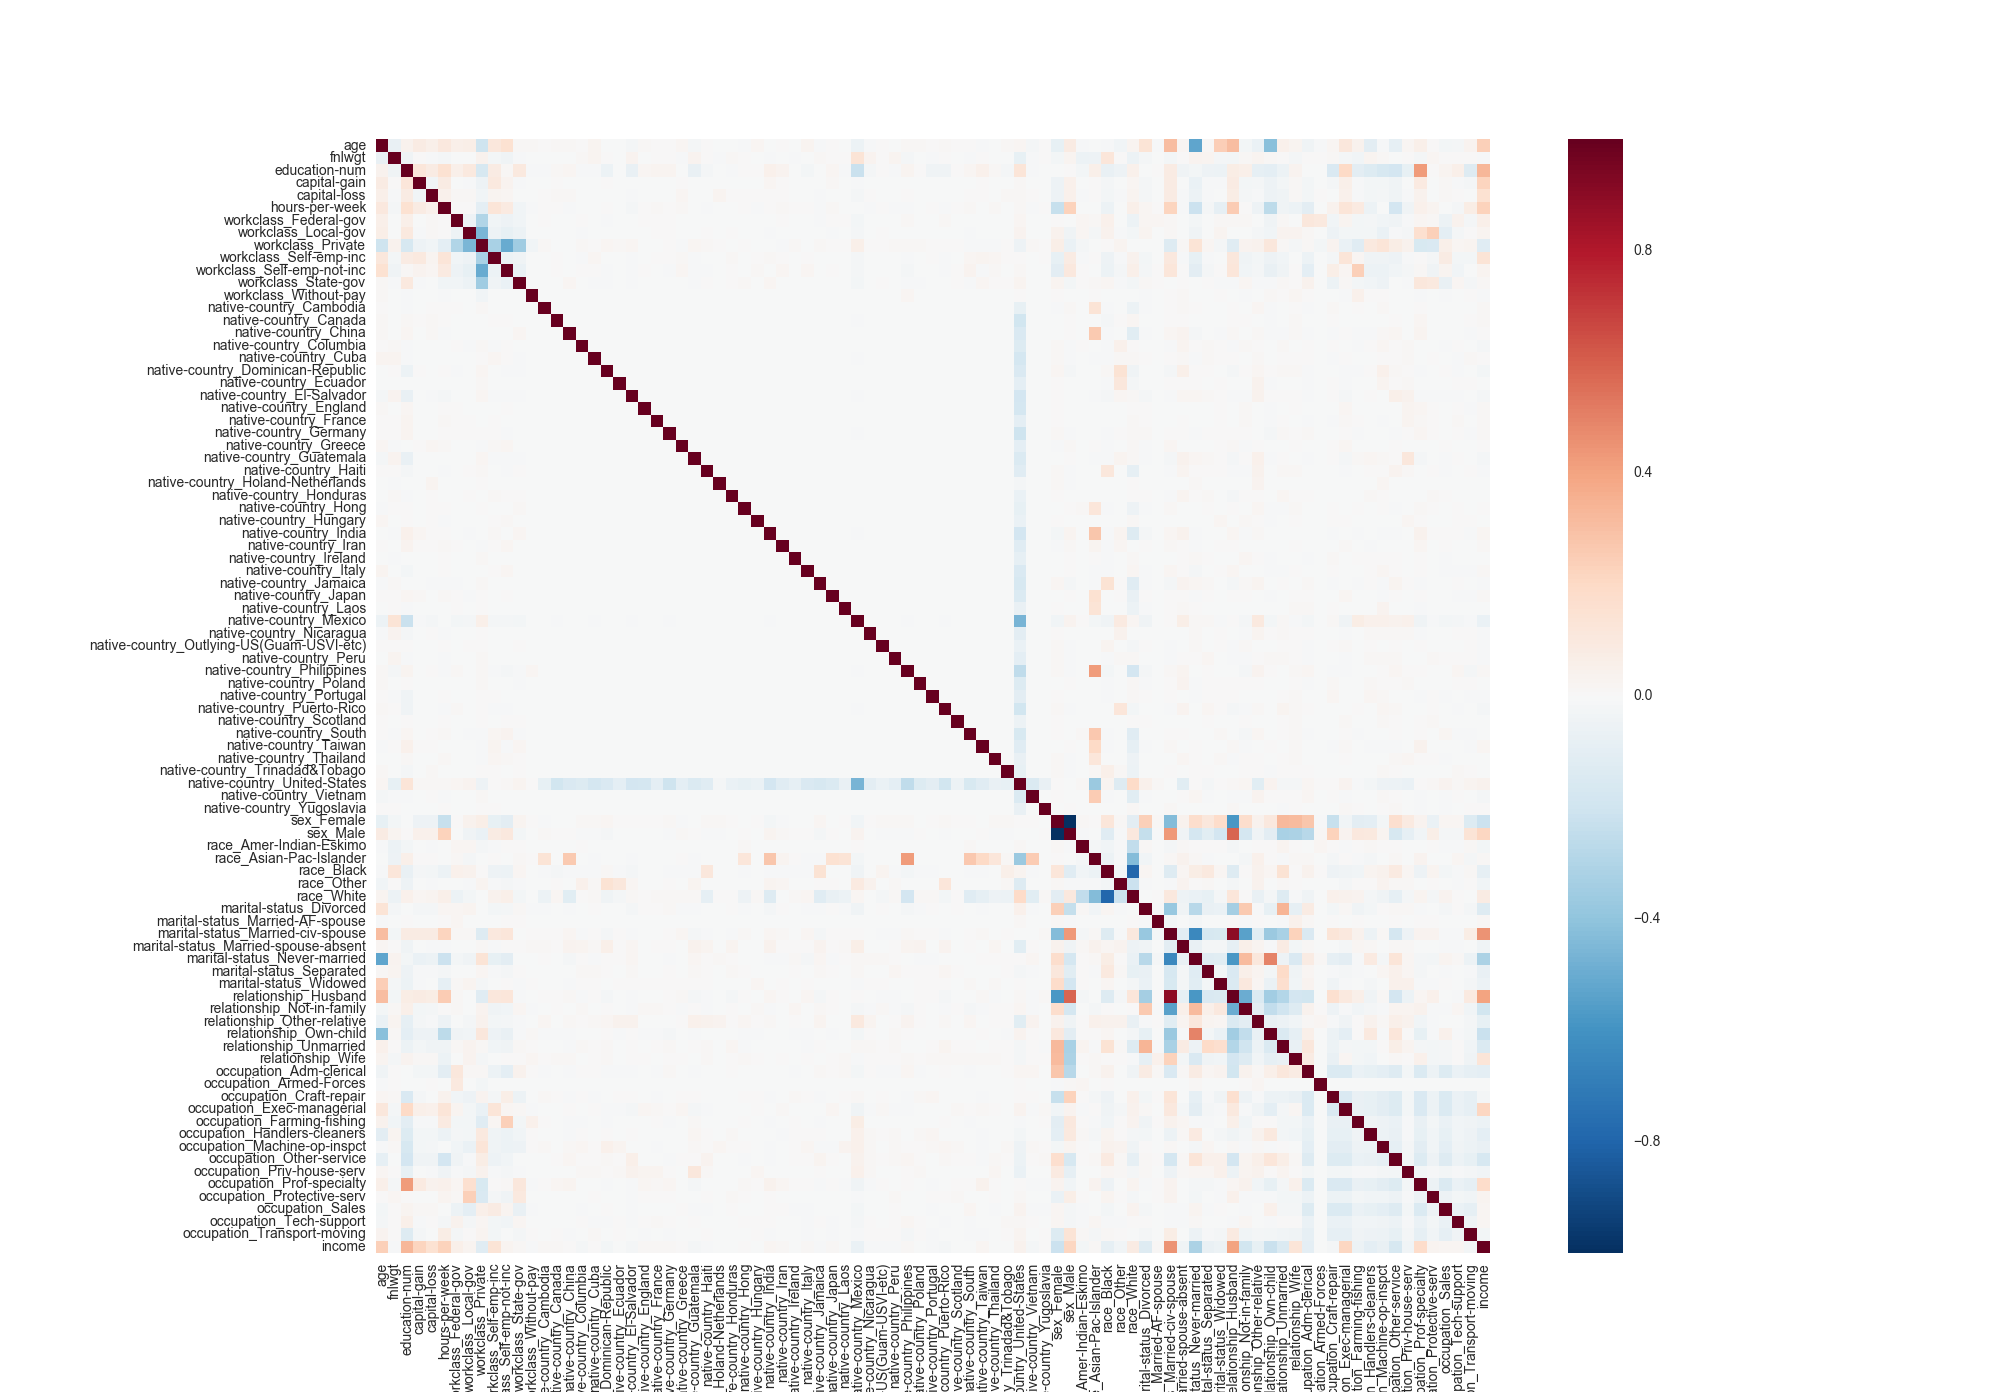
\includegraphics[width=1.3\textwidth]{figures/experiment/correlation_big}
%		\caption{Correlation matrix of the attribute values of the adult dataset}
%		\label{fig:adult_correlation_big}
%	\end{center}
% \end{figure}


\begin{figure}[!t]
	\begin{center}
		\vspace{-1.0cm}
    	\hspace*{-0.8cm}
		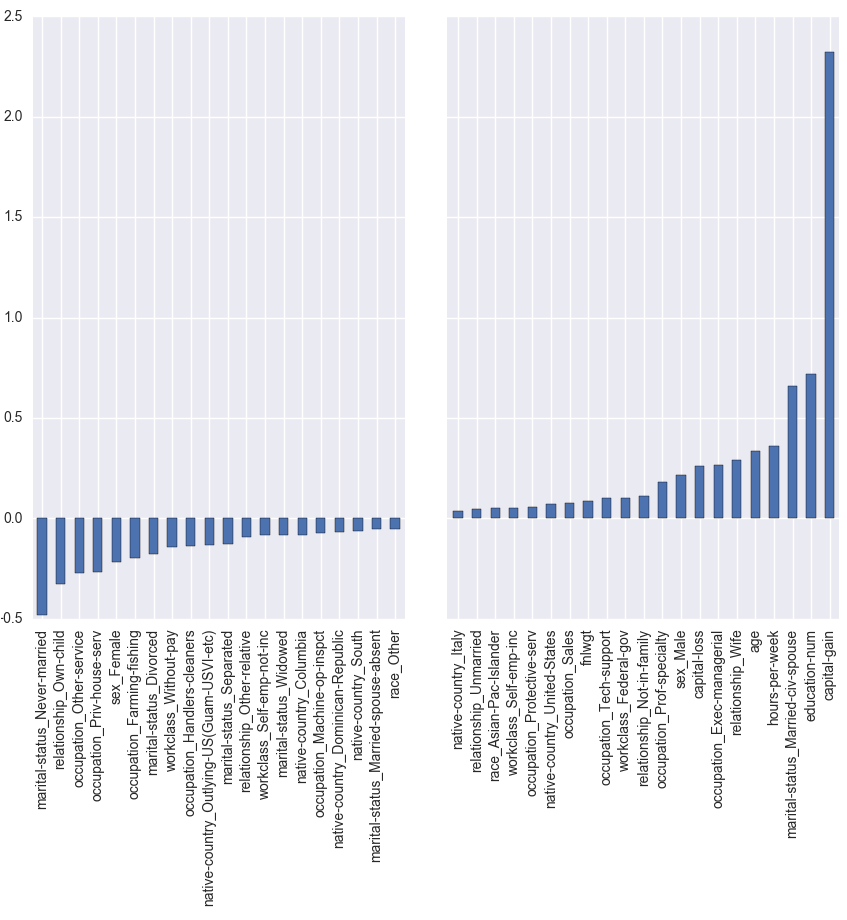
\includegraphics[width=1.1\textwidth]{figures/experiment/important_columns_cut}
		\caption{The attribute values of the adult dataset which contribute most positively / negatively to the classification result. The columns to the right strongly indicate a yearly income of above 50k, whereas the columns to the outer left indicate a yearly income of below 50k. The least significant columns in the middle part were cut out.}
		\label{fig:adult_important_columns}
	\end{center}
\end{figure}


% ==================================
%		RESULTS & DISCUSSION
% ==================================
\section{Results \& Discussion}
\label{sect:results}

We expected a steady decline in the quality of classification results over all three scenarios: 1) anonymization of datasets, 2) perturbation by selectively deleting attribute values of positive significance w.r.t the result, 3) perturbation by selectively deleting attribute values of negative significance w.r.t the result.

The actual results satisfied our expectations only in the first two cases, with the shape of the actual outcomes being a little bit surprising. As can be seen in Figure~\ref{fig:adult_results_anonymization}, the F1 score of all algorithms applied declines more drastically at the beginning, with more benign further losses as the $k$-factor of anonymization increases. Whereas the F1 curves for gradient boosting, linear SVC and logistic regression approximate a $1/x$ curve, the random forest classifier reacts more sensitively to even slight anonymization, but seems to stay more robust with higher values of $k$.

Considering the exact performance, Linear SVC and logistic regression yielded the worst outcomes under anonymization, which is not further surprising given their lower scores on the original input data to begin with.


\begin{figure}[!t]
	\begin{center}
		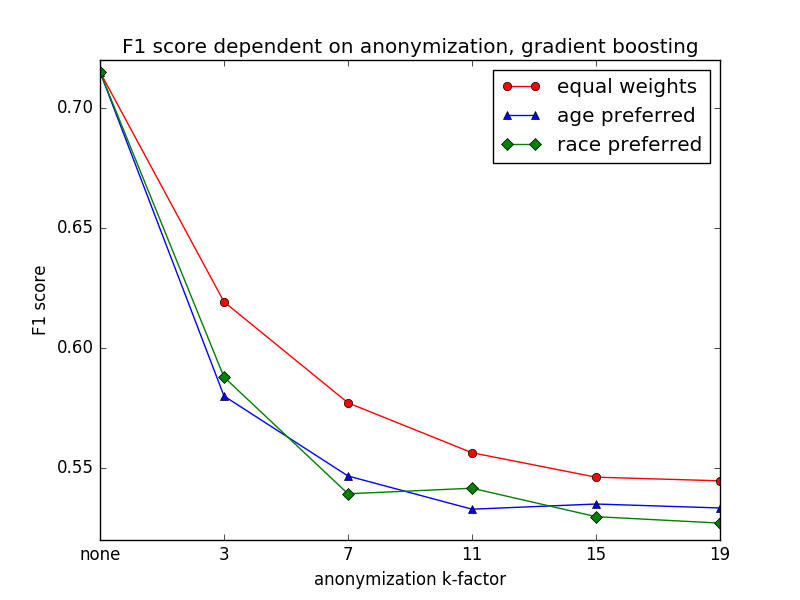
\includegraphics[width=0.49\textwidth]{figures/results/anon_gradient_boost}
		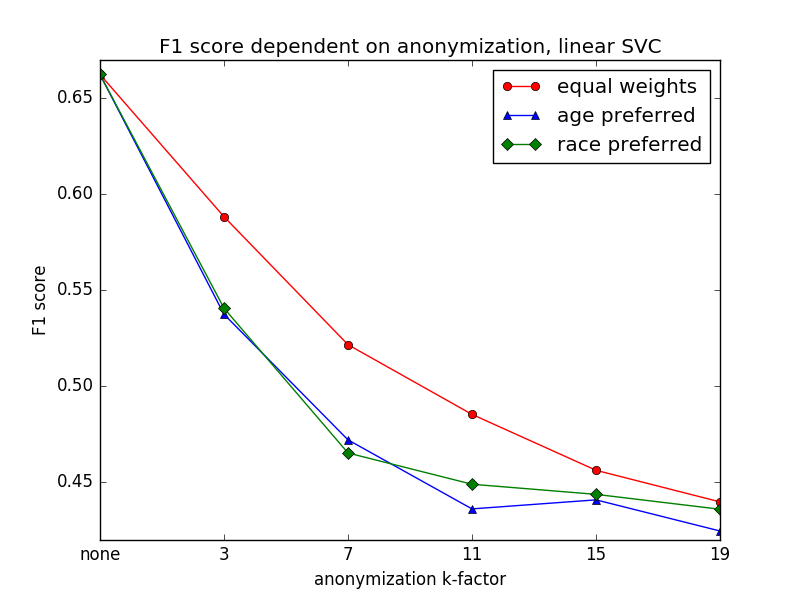
\includegraphics[width=0.49\textwidth]{figures/results/anon_linear_svc}
		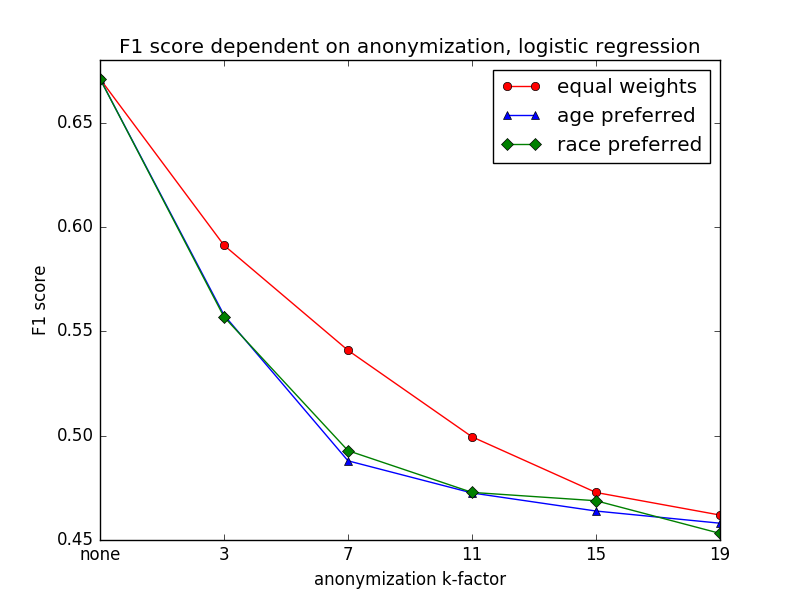
\includegraphics[width=0.49\textwidth]{figures/results/anon_logistic_regression}
		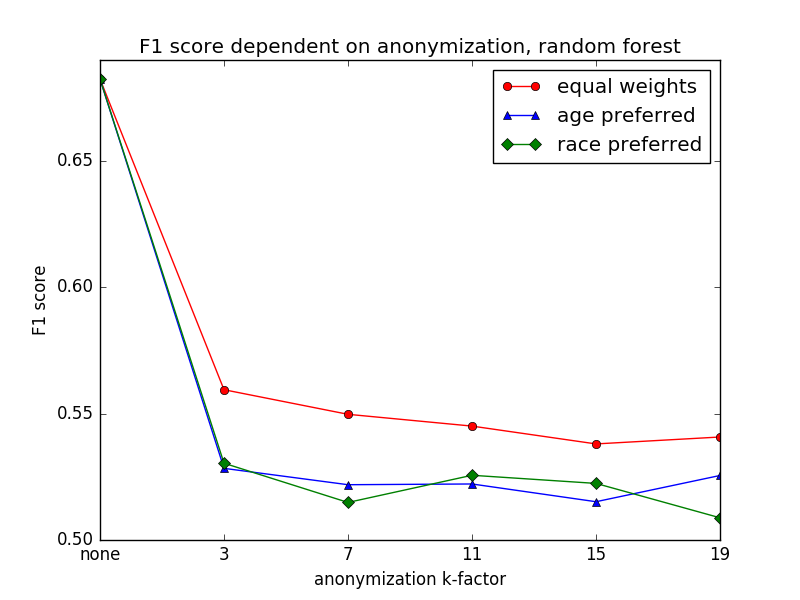
\includegraphics[width=0.49\textwidth]{figures/results/anon_random_forest}
		\caption{The impact of anonymization on the F1 score of different classifiers}
		\label{fig:adult_results_anonymization}
	\end{center}
\end{figure}


As far as the second case is concerned (Figure~\ref{fig:adult_results_perturbation_top}), our experiments showed the expected drop in algorithm performance, although the impact shows a different behavior: In the case of deleting rows with capital gain values of $>$ 2000 US-Dollars, the decline seems to be linear, whereas for the other two attribute values the performance seems to collapse with higher rates of erasure. Moreover, this behavior is more or less the same for all applied algorithms. This seems to point to the fact that especially significant attribute values can uphold a good performance even in low quantities.


\begin{figure}[!t]
	\begin{center}
		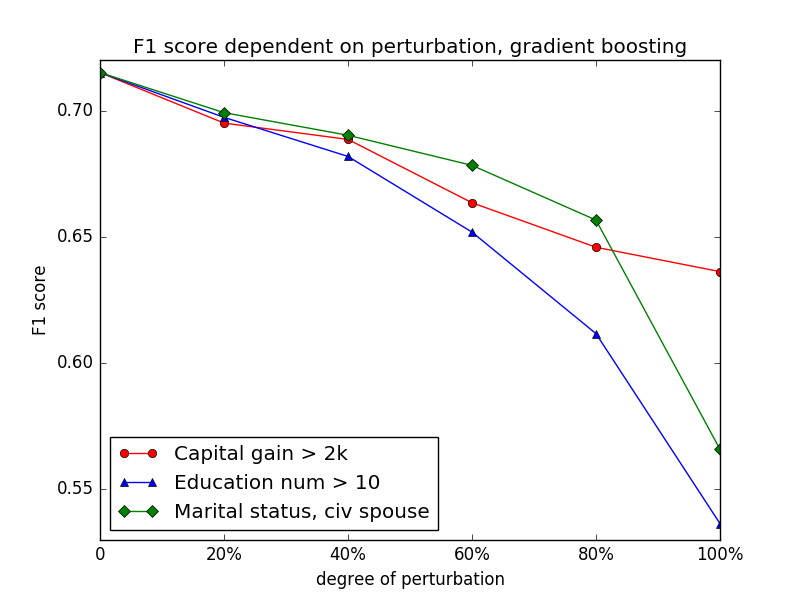
\includegraphics[width=0.49\textwidth]{figures/results/perturb_gradient_boost}
		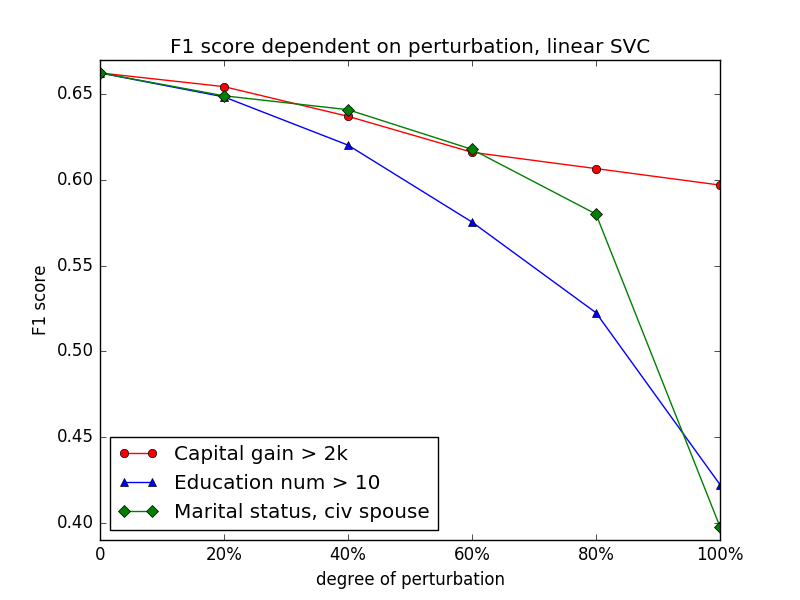
\includegraphics[width=0.49\textwidth]{figures/results/perturb_linear_svc}
		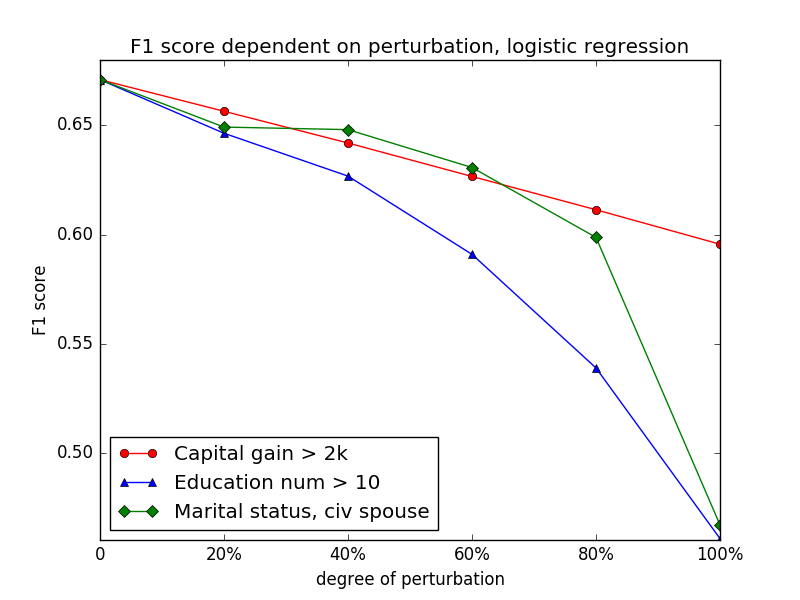
\includegraphics[width=0.49\textwidth]{figures/results/perturb_logistic_regression}
		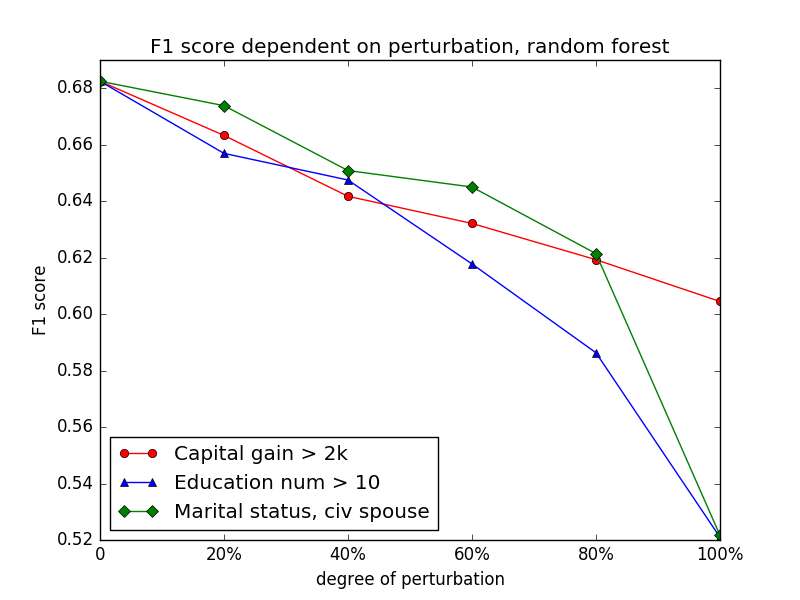
\includegraphics[width=0.49\textwidth]{figures/results/perturb_random_forest}
		\caption{The impact of perturbation (selectively deleting quantiles of rows containing one of the TOP 3 positively contributing attributes) on the F1 score of different classifiers}
		\label{fig:adult_results_perturbation_top}
	\end{center}
\end{figure}


The only real surprise occurred with applying our classifiers to the datasets perturbed by deleting percentages of attribute values indicating a low yearly income (Figure~\ref{fig:adult_results_perturbation_bottom}). As with scenario 2 we expected to see a progressive decline in performance - but with all classifiers the results either stayed approximately the same or even improved in some cases (please consider the extremely narrow scale in the respective plots). As the classification score is dependent on (in-)correctly classifying both positive and negative outcomes, this seems rather surprising and will require further investigation.


\begin{figure}[!t]
	\begin{center}
		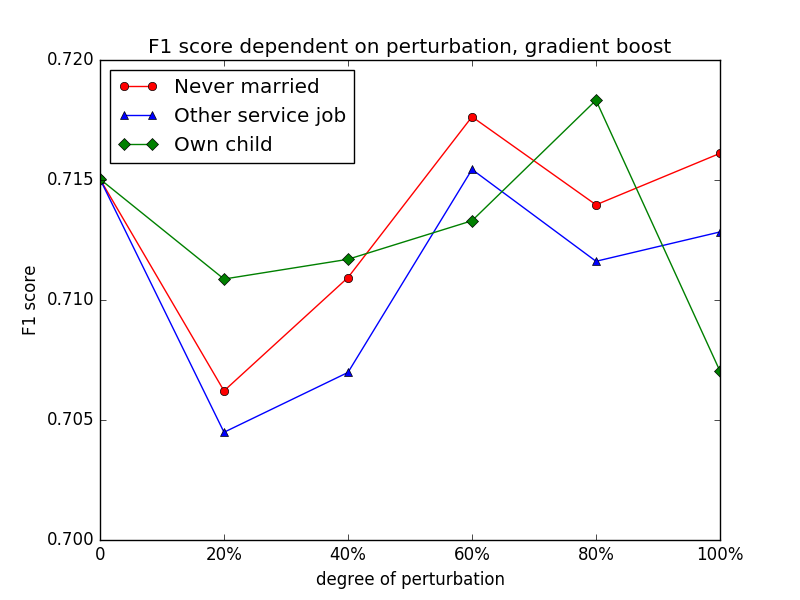
\includegraphics[width=0.49\textwidth]{figures/results/perturb_gradient_boost_bottom}
		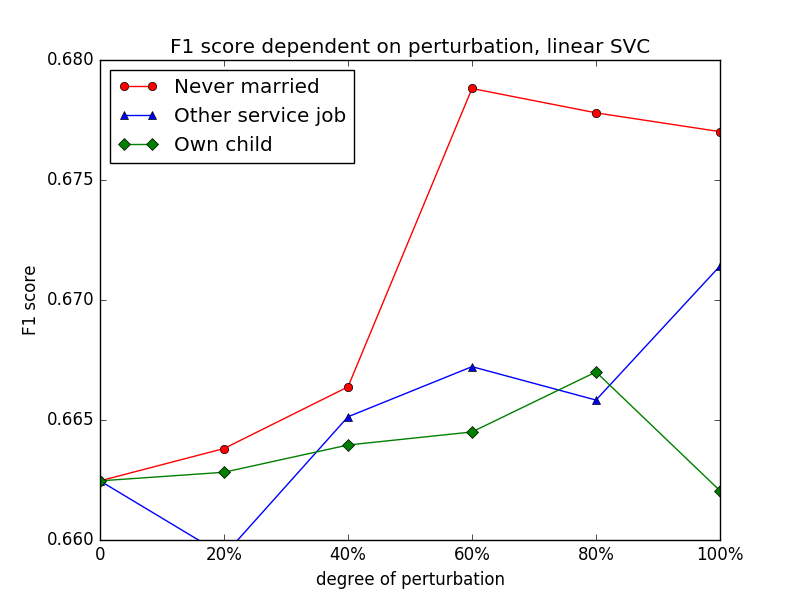
\includegraphics[width=0.49\textwidth]{figures/results/perturb_linear_svc_bottom}
		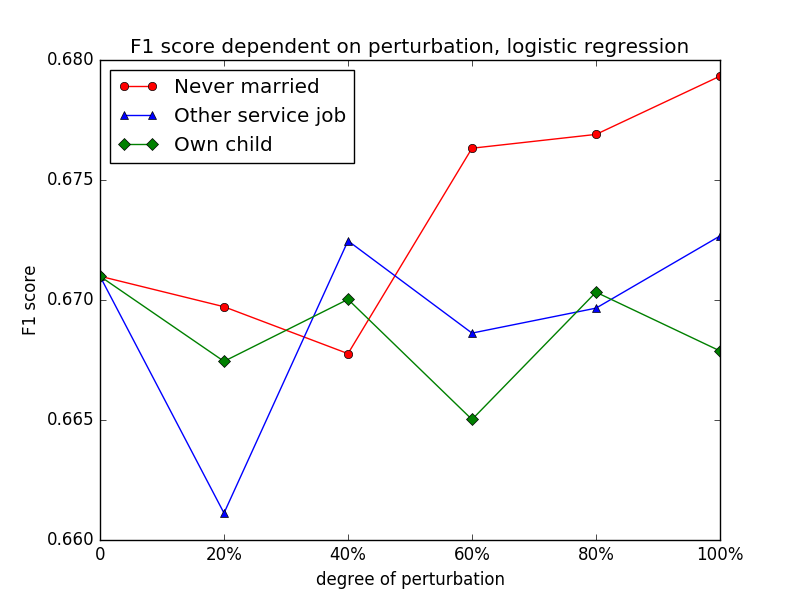
\includegraphics[width=0.49\textwidth]{figures/results/perturb_logistic_regression_bottom}
		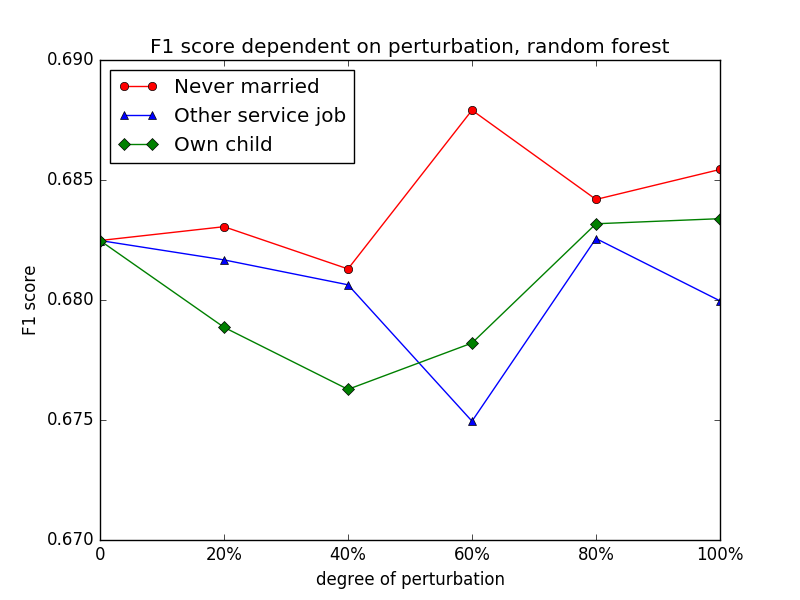
\includegraphics[width=0.49\textwidth]{figures/results/perturb_random_forest_bottom}
		\caption{The impact of perturbation (selectively deleting quantiles of rows containing one of the TOP 3 negatively contributing attributes) on the F1 score of different classifiers}
		\label{fig:adult_results_perturbation_bottom}
	\end{center}
\end{figure}


% ==================================
%			OPEN PROBLEMS
% ==================================
\section{Open problems Future challenges}
\label{sect:op_fc}

\begin{itemize}
	\item \textbf{Explain the unexpected behavior} for the datasets perturbed by selectively deleting rows containing the TOP 3 negatively contributing attribute values.
	
	\item \textbf{Find a natural dataset} which already contains a graph structure emerged in the real-world rather than a graph generator. We assume that for many modern applications the experiments conducted in this work would be highly relevant to social network analysis and anonymization, and we are planning to conduct such a research effort in a sequel to this investigation.
	
	\item \textbf{Consider the structural information loss} on a suitable real-world graph and re-apply our methodology to that data-structure. Once realistic results have been obtained, the effects of the same algorithm on artificially generated graphs might be examined, offering another perspective on the information content / structure introduced into datasets by different types of such generators.
	
	\item \textbf{Analyze the exact influence} different kinds of information loss due to anonymization / perturbation have on the different algorithms. In this work, we have only chosen a series of classifiers to demonstrate our approach. However, other classes of machine learning algorithms might yield interesting results as well, and we are motivated to conduct such future research ourselves.
	
	\item \textbf{Interactive machine learning}. We have, amongst other settings, experimented with different weight vectors in our approach regarding anonymization. However, such parameters do not easily lend themselves to be produced by an algorithm, since minimizing an artificial metric of information loss  does not produce safe datasets in itself. Moreover, data utility is highly dependent on the specific area of application; therefore choosing parameters with regard to the particular demographic and cultural clinical environment is best done by a human agent. The problem of (k-)anonymization thus represents a natural application domain for interactive Machine Learning (iML) with a human-in-the-loop \cite{Holzinger:2016:iML}, \cite{Kieseberg:2016:Doctor-in-the-Loop}, \cite{iMLExperiment}. The authors will strive to design and implement such experiments in the future.
\end{itemize}


% ==================================
%			CONCLUSION
% ==================================
\section{Conclusion}
\label{sect:conclusion}

This paper examined the question of how different ways of perturbing or anonymizing knowledge bases would influence the results of machine learning algorithms applied to those datasets. We have seen that newly introduced regulations (inside the European Union) as well as data privacy concerns of database owners naturally lead to the challenge of minimizing the cost / efficiency impact of those requirements not only on the technical, but also the machine learning infrastructure of affected businesses and organizations. Consequently, we conducted a series of experiments to simulate the decline in the F1 score of several classification algorithms on an established dataset. Our results show that selective deletion of valuable data items is less destructive than general anonymization, so that complying with regulations concerning the "right to be forgotten" is still preferable to taking preemptive steps to de-identify personal information in databases. Our results are highly selective however and should be corroborated by applying a wider spectrum of algorithms to larger, more diverse datasets.


\bibliographystyle{plain}
\bibliography{references}

\end{document}


% \begin {comment}
% \section{Glossary and Key Terms}
% NOTE: this section may not to be used for a conference
% \textbf{Note: This is only for use when producing a Springer LNCS SOTA State-of-the-Art-Analysis paper}
% \\[0,2cm]
% \emph{SaNGreeA} is the abbreviation for Social Network Greedy Anonymization, which describes an anonymization algorithm which takes into account information loss as well as structural loss (from anonymizing the neighborhood of a network node). It is said to be greedy as it uses greedy clustering under the hood in order to avoid having to sift through an exponential solution space to find an optimum.
% \end{comment}
